\documentclass[10pt, a4paper]{article}

\usepackage[english]{babel}
\usepackage{polski}
\usepackage[utf8]{inputenc}
\usepackage{graphicx}
\usepackage{float}
\title{Rozwiązanie zadania 2 z zestawu 3 z "Projektowania obiektowego oprogramowania"}
\author{Mateusz Małowiecki}
\begin{document}
\maketitle
\section*{Polecenie}
Dokonać analizy projektu obiektowego pod
katem zgodności z zasadą SRP. Zaproponować zmiany. Narysować diagramy klas przed i
po zmianach. Zaimplementować działający kod dla przykładu przed i po zmianach.
\begin{verbatim}
public class ReportPrinter {
   public string GetData();
   public void FormatDocument();
   public void PrintReport();
}

\end{verbatim}
Ile klas docelowo powstanie z takiej jednej klasy? Dlaczego akurat tyle? Czy refaktoryzacja klasy naruszającej SRP oznacza automatycznie, że każda metoda powinna trafić do
osobnej klasy?

\section*{Rozwiązanie}
\subsection*{Dokonać analizy projektu obiektowego pod
katem zgodności z zasadą SRP}
Korzystamy z testu odpowiedzialności:
\begin{verbatim}
+ReportPrinter drukuje raport sam
?ReportPrinter formatuje dokument sam
?ReportPrinter pobiera dane sam
\end{verbatim}
Widzimy teraz, że o ile drukowanie raportu jest odpowiednią odpowiedzialnością dla klasy ReportPrinter, to dwa pozostałe zadania nie są związane z drukowaniem. Jest to zatem naruszenie zasady SRP (klasa ReportPrinter ma wiele niepowiązanych ze sobą odpowiedzialności).
\subsection*{Zaproponować zmiany}
Rozdzielamy klasę ReportPrinter na klasy z pojedynczymi odpowiedzialnościami.
\subsection*{Narysować diagramy klas przed i po zmianach.}
Diagram przed:
\begin{figure}[H]
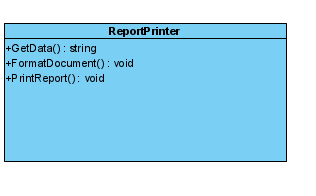
\includegraphics{Before_diagram}
\end{figure}
Diagram po:
\begin{figure}[H]
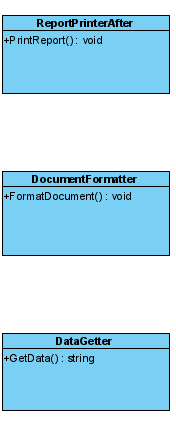
\includegraphics{After_diagram}
\end{figure}
\subsection*{Zaimplementować działający kod dla przykładu przed i po zmianach.}
Kod znajduje się w plikach "POO\_L3\_Z2\_After.cs" i "POO\_L3\_Z2\_Before.cs". W pliku "POO\_L3\_Z2\_Test.cs" znajdują się testy.
\subsection*{Ile klas docelowo powstanie z takiej jednej klasy? Dlaczego akurat tyle? Czy refaktoryzacja klasy naruszającej SRP oznacza automatycznie, że każda metoda powinna trafić do osobnej klasy?}
Docelowo powstaną trzy klasy, gdyż klasa początkowa miała trzy różne odpowiedzialności. Refaktoryzacja klasy nie oznacza, że każda metoda trafi do osobnej klasy, tylko że każda odpowiedzialność powinna zostać przypisana pojedynczej klasie. Metody związane z jedną odpowiedzialnością nie powinny być rozdzielane pomiędzy wiele klas.
\end{document}